\subsection{Regular Expressions in Streaming}
\begin{frame}
  \centering
  {\Large Streaming Regular Expression Membership and Pattern Matching}

  \bigskip
  {\large SODA'22}\\
  \bigskip
  
\includegraphics{pictures/mindmap/regexp.png}

  \bigskip
  Bartłomiej Dudek, Paweł Gawrychowski, Tatiana Starikovskaya
\end{frame}

\begin{frame}{Streaming pattern matching}
    \begin{mylemblock}{Porat and Porat, FOCS'09}
    $\Oh(\log m\cdot \log n)$ bits of space, $\Oh(\log m)$ time per position.
    \end{mylemblock}


    \bigskip
    \bblue{Main idea:} Given an algorithm $\mathcal{A}_{k}$ which generates all occurrences of
    $P[1..2^{k}]$, we will develop a new algorithm
    $\mathcal{A}_{k+1}$ which generates all occurrences of $P[1..2^{k+1}]$ using just $\Oh(\log n)$ bits of additional memory.
    \pause
    \medskip
    \begin{overlayarea}{\textwidth}{3.5cm}
    \only<2->{
    \begin{center}
    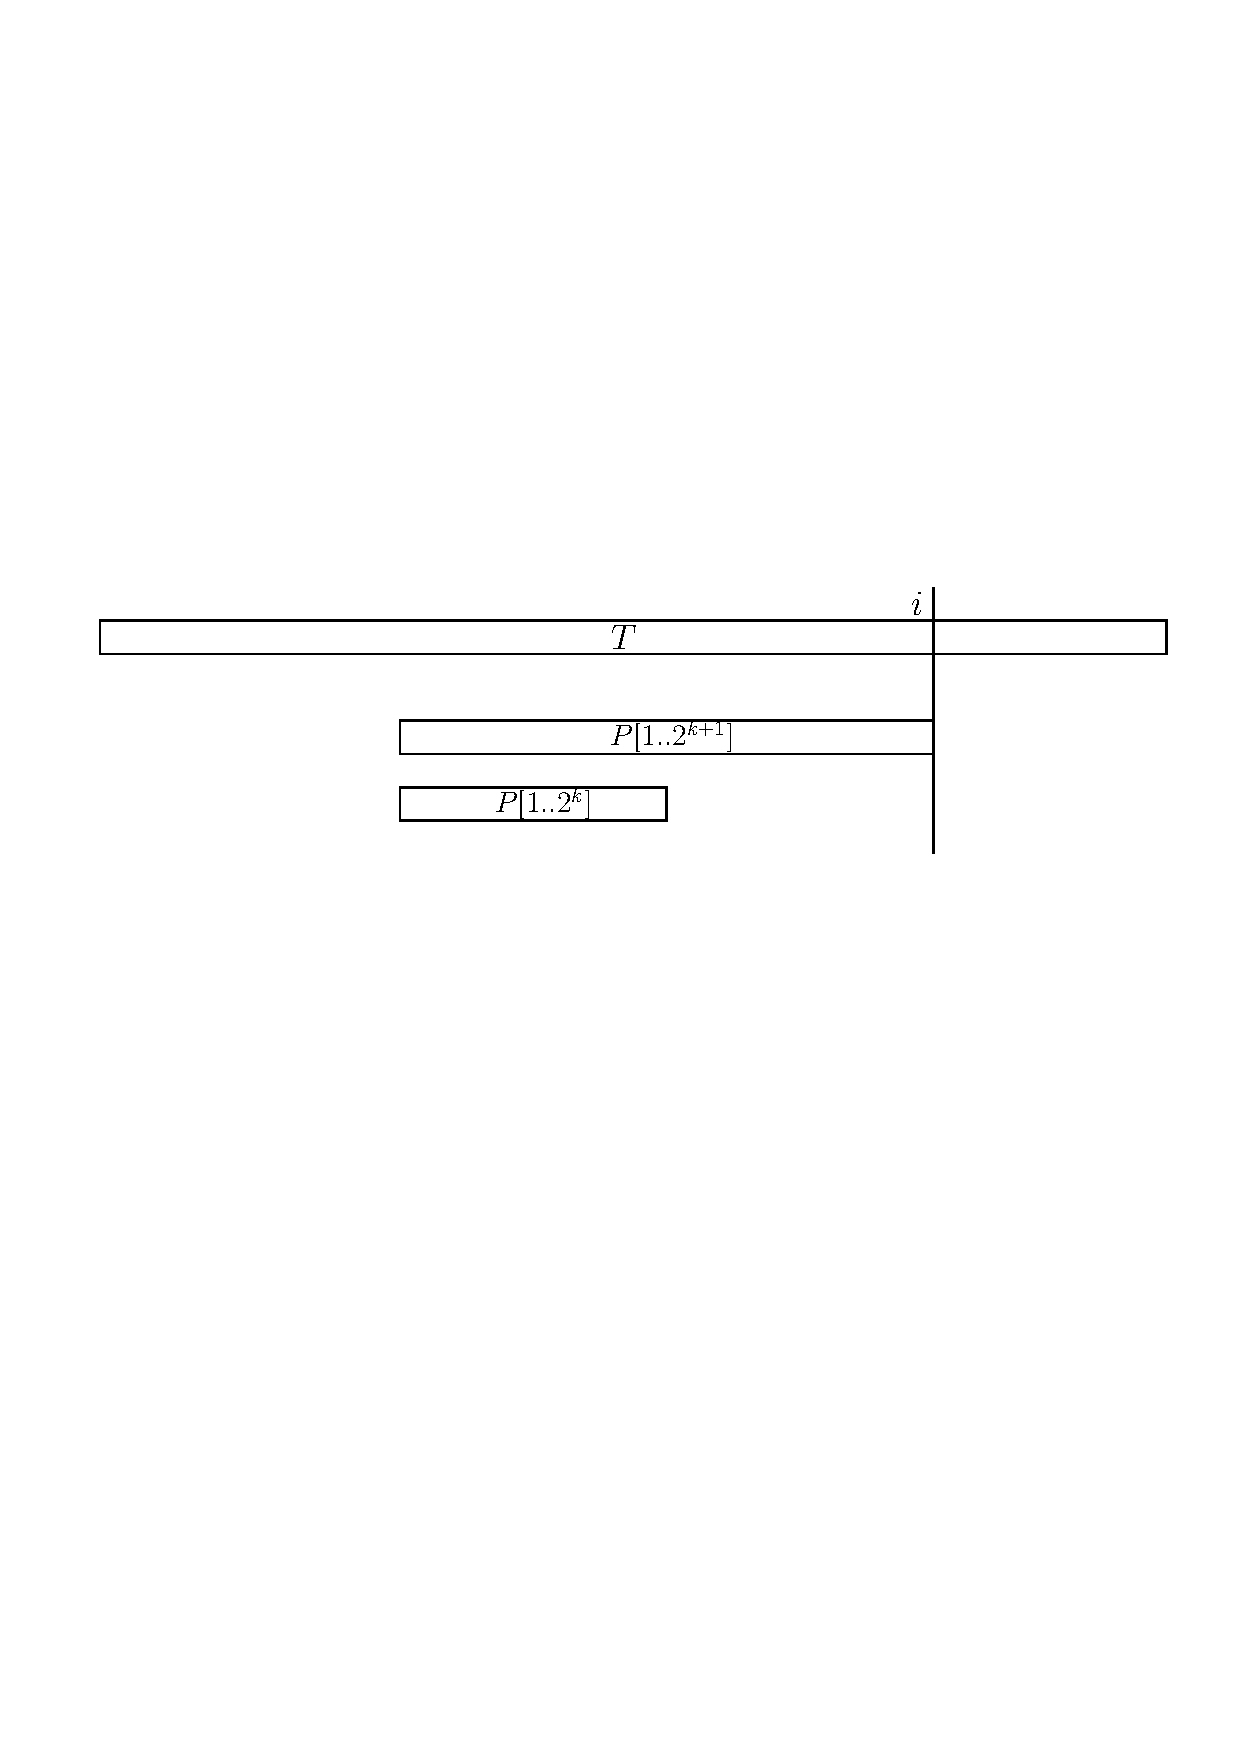
\includegraphics[width=0.7\textwidth]{pictures/more}
    \end{center}
    }
    \end{overlayarea}
    \only<3->{\centering \textcolor{red}{\textbf{But...}}\beamermathcolor{red} What if we have may occurrences of $P[1..2^{k}]$ in the window of size $2^{k+1}$ ?}
    \end{frame}
    
    
    %%%%%%%%%%%%%%%%%%%%%%%%%%%%%%%%%%%%%%%%%%%%%%%%%%%%%%%%%
    
    \begin{frame}
    
    {\beamermathcolor{red} What if we have may occurrences of $P[1..2^{k}]$ in the window of size $2^{k+1}$ ?}\pause
    
    \begin{center}
    \begin{tikzpicture}[scale=0.3]
            \node [style=none] (0) at (-13.5, 1) {};
            \node [style=none] (1) at (-13.5, 0) {};
            \node [style=none] (2) at (8.5, 0) {};
            \node [style=none] (3) at (8.5, 1) {};
            \node [style=none] (4) at (-13.5, 1) {};
            \node [style=none] (5) at (8.5, 1) {};
            \node [style=none] (6) at (-13.5, 1) {};
            \node [style=none] (7) at (8.5, 1) {};
            \node [style=none] (8) at (8.5, 1) {};
            \node [style=none] (9) at (6, 2) {};
            \node [style=none] (10) at (6, -1) {};
            \node [style=none] (11) at (5.5, 1.5) {};
            \node [style=none] (12) at (6.5, 1.5) {\small{$i$}};
            \node [style=none] (13) at (5.5, 1.5) {};
            \node [style=none] (16) at (-11.75, 0.5) {\small{$T$}};
            \node [style=none] (17) at (-2, 2) {};
            \node [style=none] (18) at (-2, 2) {};
            \node [style=none] (19) at (2, 2.5) {};
            \node [style=none] (20) at (2, 2.7) {\small{$2^{k+1}$}};
            \node [style=none] (21) at (-2, -0.25) {};
            \node [style=none] (22) at (2, -0.25) {};
            \node [style=none] (23) at (2, -1.25) {};
            \node [style=none] (24) at (-2, -1.25) {};
            \node [style=none] (26) at (0, -0.75) {\tiny{$P[1..2^k]$}};
            \node [style=none] (27) at (-1, -1.5) {};
            \node [style=none] (28) at (3, -1.5) {};
            \node [style=none] (29) at (3, -2.5) {};
            \node [style=none] (30) at (-1, -2.5) {};
            \node [style=none] (33) at (0, -2.75) {};
            \node [style=none] (34) at (4, -2.75) {};
            \node [style=none] (35) at (4, -3.75) {};
            \node [style=none] (36) at (0, -3.75) {};
            \node [style=none] (37) at (-2, -4) {};
            \node [style=none] (38) at (-1, -4) {};
            \node [style=none] (39) at (0, -4) {};
            \node [style=none] (40) at (1, -4) {};
            \node [style=none] (41) at (2, -4) {};
            \node [style=none] (42) at (3, -4) {};
            \node [style=none] (43) at (4, -4) {};
            \node [style=none] (44) at (-1, -4) {};
            \node [style=none] (45) at (0, -4) {};
            \node [style=none] (46) at (0, -4) {};
            \node [style=none] (47) at (1, -4) {};
            \node [style=none] (48) at (2, -4) {};
            \node [style=none] (49) at (1, -4) {};
            \node [style=none] (50) at (2, -4) {};
            \node [style=none] (51) at (2, -4) {};
            \node [style=none] (52) at (3, -4) {};
            \node [style=none] (53) at (4, -4) {};
            \node [style=none] (54) at (3, -4) {};
            \node [style=none] (55) at (4, -4) {};
            \draw (6.center) to (8.center);
            \draw (6.center) to (1.center);
            \draw (1.center) to (2.center);
            \draw (8.center) to (2.center);
            \draw [in=90, out=-90] (9.center) to (10.center);
            \draw (21.center) to (22.center);
            \draw (22.center) to (23.center);
            \draw (21.center) to (24.center);
            \draw (24.center) to (23.center);
            \draw (27.center) to (28.center);
            \draw (28.center) to (29.center);
            \draw (27.center) to (30.center);
            \draw (30.center) to (29.center);
            \draw [style=arrow] (18.center) to (9.center);
            \draw (33.center) to (34.center);
            \draw (34.center) to (35.center);
            \draw (33.center) to (36.center);
            \draw (36.center) to (35.center);
            \only<2->{
            \draw [bend right=90, looseness=1.50] (37.center) to (38.center);
            \draw [bend right=90, looseness=1.50] (44.center) to (45.center);
            \draw [bend right=90, looseness=1.50] (46.center) to (47.center);
            \draw [bend right=90, looseness=1.50] (49.center) to (50.center);
            \draw [bend right=90, looseness=1.50] (51.center) to (52.center);
            \draw [bend right=90, looseness=1.50] (54.center) to (55.center);}
    \end{tikzpicture}
    \end{center}
    
    \pause
    \textcolor{red}{Then there is periodicity !} \pause 
    The occurences can be stored efficiently:\pause
    \begin{itemize}
    \pause
    \item The start, the period, and the number of repetitions
    \pause
    \item The fingerprint of the prefix of the text up to the start of the progression and the fingerprint of the period
    \end{itemize}
    
    \medskip
    \pause
    
    {
        \beamermathcolor{red}
        \alert{$\Oh(\log n)$ bits of space per level!} \pause \\ 
        \footnotesize{Correctness: if $P$ occurs, all $\log m$ prefixes will be there too and be detected w.h.p.}
    }

\end{frame}

\begin{frame}{Circuit framework}
    $$C_k[u,v][d]=\bigvee_{\substack{w\in V(G) \\  i\in \{0,\ldots,d\}}} C_{k-1}[u,w][i] \wedge C_{k-1}[w,v][d-i]$$
    
    \pause 
     
    \begin{block}{Lokshtanov and Nederlof, STOC'10; Bringmann, SODA'17}
    Consider a circuit $C$ with every gate being an addition or convolution gate and computing a vectors of the same length.
    Assuming that no convolution gate overflows,
    we can efficiently compute an entry of the output vector in space depending on the size of the circuit
    (and not the length of the vectors).
    \end{block}
    \pause
    
    \begin{alertblock}{}
    We remove the dependency on the Extended Riemann Hypothesis, replacing it with an application of the Bombieri--Vinogradov theorem.\\ 
    %\pause
    %(a major result of analytic number theory, obtained in the mid-1960s, concerning the distribution of primes in arithmetic progressions)
    \end{alertblock}
    
\end{frame}
    